\documentclass{article}
\usepackage{amsmath}
\usepackage{algorithm}
\usepackage{algpseudocode}
\usepackage{listings, xcolor}
\usepackage{graphicx,float,wrapfig}
\newcommand{\Class}{Operation System}
\newcommand{\ClassInstructor}{Wei Xu}
\newcommand{\Break}{\State \textbf{break} }

% Homework Specific Information. Change it to your own

% In case you need to adjust margins:
\topmargin=-0.45in      %
\evensidemargin=0in     %
\oddsidemargin=0in      %
\textwidth=6.5in        %
\textheight=9.0in       %
\headsep=0.25in         %

% Setup the header and footer                                 %

%%%%%%%%%%%%%%%%%%%%%%%%%%%%%%%%%%%%%%%%%%%%%%%%%%%%%%%%%%%%%
% Some tools

%%%%%%%%%%%%%%%%%%%%%%%%%%%%%%%%%%%%%%%%%%%%%%%%%%%%%%%%%%%%%


%%%%%%%%%%%%%%%%%%%%%%%%%%%%%%%%%%%%%%%%%%%%%%%%%%%%%%%%%%%%%
% Make title
\title{Project 1 - Initial Design Document}
\author{Chen Lijie\\ 2013011313\and
	Fan Haoqiang\\ 2011012357\and
	Bi Ke\\ 2011012360}
\date{}
%%%%%%%%%%%%%%%%%%%%%%%%%%%%%%%%%%%%%%%%%%%%%%%%%%%%%%%%%%%%%

\begin{document}
	\maketitle
	\tableofcontents
	\section{Our git Repository}
	\texttt{https://github.com/wjmzbmr/nachos}
	\section{Implementation of KThread.join()}
	
	\subsection{Correctness Invariants}
	
	\begin{itemize}
		\item A thread should not join to itself and a finished thread should not join to other threads.
		\item The method need to be made atomic, by disabling interrupting at first, and restore it when the method returns.
		\item Whether being joined or not, a thread must finish executing normally.
	\end{itemize}

	\subsection{Declaration}
	\begin{itemize}
		\item In class KThread, add a member variable waiterQueue(a queue of Thread), which stores the joined threads.
		
		\item Modification in KThread.join() and Thread.finish().
    \end{itemize}
	
	\subsection{Description}
	
	The pseudocodes for modifications of both methods are listed below.
	
	\begin{algorithm}[H]
		\begin{algorithmic}
			\Procedure {join()}{}
   				\State Disable Interruption
				\If{this != currentThread and this.status != statusFinished}
					\State add currentThread to waiterQueue
					\State Let the currentThread sleeps
				\EndIf
				\State Restore Interruption
			\EndProcedure
		\end{algorithmic}
	\end{algorithm}
	
	\begin{algorithm}[H]
		\begin{algorithmic}
			\Procedure {finish()}{}
				\State ...
				\State currentThread.status = statusFinished
				\State Wake up threads in waiterQueue.
				\State sleep()
			\EndProcedure
		\end{algorithmic}
	\end{algorithm}
	
	
	\subsection{Testing strategy}
	
	We plan to make the following tests.
	\subsubsection*{1. Standard Case Testing}
	Make a thread, joined it to another one, and check whether it running order is the same as our expectation.
	
	\subsubsection*{2. A thread joined to many other threads}
	Make a thread, joined it to several other threads and check whether the result is the same as our expectation.
	
	\subsubsection*{3. A thread be joined by many other threads}
	Make a thread, let it be joined by several other threads and check whether the result is the same as our expectation.
	
	\subsubsection*{4. Corner Case Testing}
	Make some threads be joined to itself, and join some finished threads to other threads to see whether or not those corner cases are correctly handled.
	
	\newpage
	
	\section{Another Implementation of Condition Variable}
	
	\subsection{Correctness Invariants}
	
	\subsubsection*{sleep()}
	\begin{itemize}
		\item The current thread must hold the lock before the method, and get the lock again after the method.
		
		\item The operation that releases the lock and put the current thread into the waiting queue  must be atomic.
	\end{itemize}
	
	\subsubsection*{wake()}
	\begin{itemize}
		\item The current thread must hold the lock before the method.
			
		\item The operation that wake up a thread which called sleep() before must be atomic.
	\end{itemize}
	
	\subsubsection*{wakeAll()}
	\begin{itemize}
		\item The current thread must hold the lock before the method.
		
		\item The operation that wake up all the threads which called sleep() before must be atomic.
	\end{itemize}
	
	\subsection{Declaration}
	
	\begin{itemize}
		\item In class Condition2, add a member variable waiterQueue(a queue of Thread), which stores the waiting threads.
		
		\item a method sleep(), same functionality as in the class Condition.
		
		\item a method wake(), same functionality as in the class Condition.
		
		\item a method wakAll(), same functionality as in the class Condition.
	\end{itemize}
	
	\subsection{Description}
	
	Following are the pseudocodes for all the methods above.
	
	\begin{algorithm}[H]
		\begin{algorithmic}
			\Procedure {sleep()}{}
				\State Lib.assertTrue(conditionLock.isHeldByCurrentThread())
				\State Disable Interruption
				\State Add currentThread to waiterQueue
				\State Release the lock
				\State let currentThread sleep
				\State Acquire the lock
				\State Restore Interruption
			\EndProcedure
		\end{algorithmic}
	\end{algorithm}
		
	\begin{algorithm}[H]
		\begin{algorithmic}
			\Procedure {wake()}{}
				\State Lib.assertTrue(conditionLock.isHeldByCurrentThread())
				\State Disable Interruption
				\If{WaiterQueue is not empty}
					\State Wake up and remove one thread in the waiterQueue.
				\EndIf
				\State Restore Interruption
			\EndProcedure
		\end{algorithmic}
	\end{algorithm}
	\begin{algorithm}[H]
		\begin{algorithmic}
			\Procedure {wakeAll()}{}
				\State Lib.assertTrue(conditionLock.isHeldByCurrentThread())
				\State Disable Interruption
				\While{WaiterQueue is not empty}
					\State Wake up and remove one thread in the waiterQueue.
				\EndWhile
				\State Restore Interruption
			\EndProcedure
		\end{algorithmic}
	\end{algorithm}
	
	\subsection{Testing strategy}
	
	\subsubsection*{1. Using Condition2 to implement the producer and consumer problem}
	
	Write a simple program which use Condition2 to implement the producer and consumer problem and check whether or not the results are meeting our expectation.
%	
	\section{Implementation of the Alarm}
	
	\subsection{Correctness Invariants}
	
	\subsubsection*{waitUntil()}
	\begin{itemize}
		\item The operation that moving the currentThread into the waiting queue and sleep it must be atomic.
	\end{itemize}
	
	\subsubsection*{timerInterrupt()}
	\begin{itemize}
		\item Every threads whose waiting time is over must be waken up.
		
		\item The operation that wakes up all those threads must be atomic.
	\end{itemize}
	
	\subsection{Declaration}
	
	\begin{itemize}
		\item A new class WaitingThread, which records a thread which are waiting together with its designated waking up time. It should be comparable by its waking up time.
		
		\item A new member priority queue waiterQueue in the class Alarm, which stores all the WaitingThread according to their waking up time, so we can retrieve the thread with minimum waking up time quickly.
		
		\item Modification in timerInterrupt().
		
		\item Modification in waitUntil().
	\end{itemize}
	
	\subsection{Description}
	
	Following are the pseudocodes for all the methods above.
	
	\begin{algorithm}[H]
		\begin{algorithmic}
			\Procedure {WaitingThread(wakeTime,Thread)}{}
				\State \Return a WaitingThread object with the given wakeTime and Thread
			\EndProcedure
		\end{algorithmic}
	\end{algorithm}
	
	\begin{algorithm}[H]
		\begin{algorithmic}
			\Procedure {waitUntil(x)}{}
				\State Disable Interruption
				\State wakeTime $ \leftarrow$ currentSystemTime + x
				\State Add WaitingThread(wakeTime,currentThread) to waiterQueue
				\State let the currentThread sleep.
				\State Restore Interruption
			\EndProcedure
		\end{algorithmic}
	\end{algorithm}
	
	\begin{algorithm}[H]
		\begin{algorithmic}
			\Procedure {timerInterrupt(x)}{}
			\State Disable Interruption
			\While{The waiterQueue is not empty}
				\State t $\leftarrow$ waiterQueue.peek()
				\If{t.wakeTime $>$ currentSystemTime}
					\Break
				\EndIf
				\State Wake t up
				\State waiterQueue.poll()
			\EndWhile		
			\State Restore Interruption
			\EndProcedure
		\end{algorithmic}
	\end{algorithm}
	
	\subsection{Testing strategy}
	
	\subsubsection*{1. Specified Ordering}
	Make many threads(around $50$), and let the $i$-th thread waitUntil with a corresponding with x=$2000 \cdot i$. 
	
	Then we check whether their are waken up at the same order.
	
	\subsubsection*{2. Specified Ordering with small x}
	Change the x in the previous test to $200$ to see what happens, note $200$ is smaller than the timer's clock ticks.
	
	\subsubsection*{3. Randomized Ordering}
	Make many threads(with varying multitude like $10$, $100$,$1000$) with randomized x.
	
	Then we check whether their waken up order meets our expectation.
%	
	\section{Implementation of the Communicator}
	
	\subsection{Correctness Invariants}
	
	\subsubsection*{speak()}
	\begin{itemize}
		\item The speaker will wait if its word are not listener by a listener.
		\item The operation that setting the spoken word must be atomic.
		\item The speaker can not setting the spoken word if it has not been taken by a listener.
	\end{itemize}
	
	\subsubsection*{listen()}
	\begin{itemize}
		\item The listener will wait if there is no set word.
		\item The operation that taking the spoken word must be atomic.
	\end{itemize}
	
	\subsection{Declaration}
	\begin{itemize}
		%\item Our solution follow the same spirit for the bounded buffer problem(Indeed it is a special case for it, so the correctness is obvious)
		\item A state variable temp, to temporarily store the spoken word.
		
		\item A lock mutex, which ensure the operation involving the word must be atomic.
		
		\item 4 variables, AS,AL,WS,WL, indicate the current number of active speaker, active listener, waiting speaker, waiting listener.
		
		\item 4 conditions variables with lock mutex, waitS for waiting speaker, waitL for waiting listener, waitToTake for the active listener who are waiting to take the word, waitTaken for the active speaker waiting for its word to be taken.
		
		\item Function speak(word), and procedure listen().
	\end{itemize}
	
	\subsection{Description}
	
	\begin{algorithm}[H]
		\begin{algorithmic}
			\Procedure {Initialize()}{}
			\State AS,AL,WS,WL $\leftarrow$ 0.
			\State Initialize mutex, and all conditions with mutex.
			\EndProcedure
		\end{algorithmic}
	\end{algorithm}
	
	\begin{algorithm}[H]
		\begin{algorithmic}
			\Procedure {speak(word)}{}
			\State mutex.acquire()
			\While{NOT (AS == 0 AND AL $>$ 0)}
				\State WS+=1
				\State waitS.sleep()
				\State WS-=1
			\EndWhile
			\State AS+=1
			\State temp $\leftarrow$ word.
			\State waitToTake.wake() 
			\State waitTaken.sleep() //waiting for word to be taken
			\State AS-=1
			\If{WS $>$ 0}
				\State waitS.wake()
			\EndIf
			\State mutex.release()
			\EndProcedure
		\end{algorithmic}
	\end{algorithm}
	
	\begin{algorithm}[H]
		\begin{algorithmic}
			\Procedure {listen()}{}
				\State mutex.acquire()
			\While{NOT (AL == 0)}
				\State WL+=1;
				\State waitL.sleep()
				\State WL-=1
			\EndWhile
			\State AL+=1
			\If{WS $>$ 0}
				\State waitS.wake();
			\EndIf
			\State waitToTake.sleep();
			\State take temp;
			\State waitTaken.wake();
			\State AL-=1;
			\If{WL $>$ 0}
				\State waitL.wake()
			\EndIf
			\State mutex.release();
			\EndProcedure
		\end{algorithmic}
	\end{algorithm}
	
	\subsection{Testing strategy}
	
	\subsubsection*{Randomized test}
	Generate some speakers and listeners randomly, and check whether the correctness conditions are met.
%	
	\section{Implementation of the PriorityScheduler}
	
	\subsection{Correctness Invariants}
	
	\begin{itemize}
		\item For the threads waiting for the same resource, the one with higher priority get the resource first, in case of a tie, the one has been waiting for longest time get it first.
		
		\item Every methods do the scheduling must be atomic.
		
		\item If a thread is waiting for a particular resource, its priority will be donated to the thread which holds that resource.
	\end{itemize}
	
	\subsection{A simple illustration}
	We know:
	
	\begin{itemize}
	\item A thread can only wait for one resource, while it may holds access to several resources.
	
	\item A resource can only be hold with one thread.
	\end{itemize}
	
	So the relation graph looks like:
	
	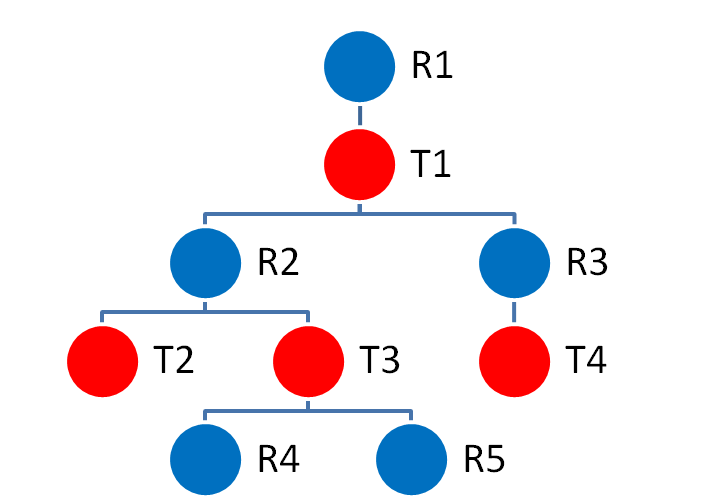
\includegraphics[width=8cm]{structure.png}
	
	And it has a tree structure, so when updating one thread's priority, we can just update the effective priority from bottom to top.
	
	This can be done with a sophisticated structure like Link-cut tree or Splay tree to maintain the DFS order of all the nodes. But since, the tree-depth are normally not very large, I think a simple brute-force update from leaf to root is sufficient.
	
	\subsection{Declaration}
	\subsubsection{Scheduler}
	
	\begin{itemize}
		\item Implementation of getPriority(), setPriority() and getEffectivePriority
	\end{itemize}
	
	\subsubsection{Kthread}
	
	\begin{itemize}
		\item Notice that the original Kthread Object has a member schedulingState, which can be used to record its scheduling state.
	\end{itemize}
	\subsubsection{PriorityThreadQueue}
	
	\begin{itemize}
		\item Make a subclass of ThreadQueue named PriorityThreadQueue. Which is supposed to maintain the threads waiting for this resource.
		
		\item A member variable resourceHolder, which points to the thread which holds the resource.
		
		\item A member variable maxPriority, which denoting the maximum effective priority in the waiterQueue, set as minimum if waiters is empty.
		
		\item A binary search tree of SchedulingState waiters contains all the waiting threads, and compare them with the priority and the enqueue Time.
		
		\item implementation of nextThread(), acquire(), waitForAccess().
	\end{itemize}
	
	\subsubsection{SchedulingState}
	
		\begin{itemize}
			
			\item member variables thread, priority, enqueueTime, effectivePriority, waitingResource which corresponding to the thread it represents, the priority of that thread, the enqueueTime of that thread, the effective priority of that thread, and the resource this thread is waiting for.
			
			\item A member variable resources implemented by a binary search tree, which holds all the resources acquired by this thread.
		\end{itemize}
	
	\subsection{Description}
	\subsubsection{Scheduler}
	\begin{algorithm}[H]
		\begin{algorithmic}
			\Procedure {getPriority(thread)}{}
			\State \Return thread.schedulingState.priority
			\EndProcedure
		\end{algorithmic}
	\end{algorithm}
	
	\begin{algorithm}[H]
		\begin{algorithmic}
			\Procedure {getEffectivePriority(thread)}{}
			\State \Return thread.schedulingState.effectivePriority
			\EndProcedure
		\end{algorithmic}
	\end{algorithm}
	
	\begin{algorithm}[H]
		\begin{algorithmic}
			\Procedure {setPriority(thread, p)}{}
			\If{p $<$ priorityMinimum OR p $>$ priorityMaximum}
				\State \Return
			\EndIf
			\State thread.schedulingState.setPriority(p)
			\EndProcedure
		\end{algorithmic}
	\end{algorithm}
	
	\subsubsection{PriorityThreadQueue}
	
	\begin{algorithm}[H]
		\begin{algorithmic}
			\Procedure {Initialize()}{}
			\State resourceHolder $\leftarrow$ null;
			\State waiters $\leftarrow$ new empty TreeSet.
			\EndProcedure
		\end{algorithmic}
	\end{algorithm}
	
	\begin{algorithm}[H]
		\begin{algorithmic}
			\Procedure {getMaxPriority()}{}
				\If{waiters.empty()}
					\State \Return priorityMinimum
				\EndIf
				\Return waiters.first().effectivePriority
			\EndProcedure
		\end{algorithmic}
	\end{algorithm}
	
	\begin{algorithm}[H]
		\begin{algorithmic}
			\Procedure {update()}{}
			\State tmp $\leftarrow$ getMaxPriority()
			\If{tmp != maxPriority}
				\If{resourceHolder}
					resourceHolder.updateResource(this,maxPriority)
				\Else
					maxPriority $\leftarrow$ tmp
				\EndIf
			\EndIf
			\EndProcedure
		\end{algorithmic}
	\end{algorithm}
	
	\begin{algorithm}[H]
		\begin{algorithmic}
			\Procedure {updateWaiter(state, EP)}{}
				waiters.remove(state)
				state.effectivePriority $\leftarrow$ EP
				watiers.add(state)
				update()
			\EndProcedure
		\end{algorithmic}
	\end{algorithm}
	
	\begin{algorithm}[H]
		\begin{algorithmic}
			\Procedure {waitForAccess(thread)}{}
			\State state $\leftarrow$ thread.schedulingState
			\State state.enqueueTime $\leftarrow$ currentTime
			\State state.waitingResource $\leftarrow$ this
			\State waiterQueue.add(state)
			\State update()
			\EndProcedure
		\end{algorithmic}
	\end{algorithm}
	
	\begin{algorithm}[H]
		\begin{algorithmic}
			\Procedure {acquire(thread)}{}
			\State state $\leftarrow$ thread.schedulingState
			\State resourceHolder $\leftarrow$ state
			\State state.addResource(this)
			\EndProcedure
		\end{algorithmic}
	\end{algorithm}
	
	\begin{algorithm}[H]
		\begin{algorithmic}
			\Procedure {nextThread()}{}
			\If{resourceHolder != null}
				\State resourceHolder.removeResource(this)
				\State resourceHolder $\leftarrow$ null
			\EndIf
			\If{waiterQueue.empty()}
				\State \Return null
			\EndIf
			\State state $\leftarrow$ waiterQueue.poll()
			\State thread $\leftarrow$ state.thread
			\State update()
			\State state.waitingResource = null
			\State state.addResource(this);
			\Return thread
			\EndProcedure
		\end{algorithmic}
	\end{algorithm}
	
	\subsubsection{SchedulingState}
	
	\begin{algorithm}[H]
		\begin{algorithmic}
			\Procedure {Initialize()}{}
			\State priority, effectivePriority $\leftarrow$ priorityDefault
			\State resources $\leftarrow$ empty TreeSet
			\State waitingResource $\leftarrow$ null
			\EndProcedure
		\end{algorithmic}
	\end{algorithm}
	
	\begin{algorithm}[H]
		\begin{algorithmic}
			\Procedure {update()}{}
			\State tmp $\leftarrow$ priority
			\If{!resources.empty()}
				\State tmp $\leftarrow$ max(tmp, resources.first().maxPriority)
			\EndIf
			
			\If{tmp != effectivePriority}
				\If{waitingResource != null}
					\State waitingResource.updateWaiter(this,tmp)
				\Else
					\State effectivePriority $\leftarrow$ tmp
				\EndIf
			\EndIf
			
			\EndProcedure
		\end{algorithmic}
	\end{algorithm}
	\begin{algorithm}[H]
		\begin{algorithmic}
			\Procedure {setPriority(p)}{}
			\State priority $\leftarrow$ p
			\State update()
			\EndProcedure
		\end{algorithmic}
	\end{algorithm}
	
	\begin{algorithm}[H]
		\begin{algorithmic}
			\Procedure {updateResource(res, maxP)}{}
			\State resources.remove(res)
			\State res.maxPriority $\leftarrow$ maxP
			\State resources.add(res)
			\State update()
			\EndProcedure
		\end{algorithmic}
	\end{algorithm}
	
	\begin{algorithm}[H]
		\begin{algorithmic}
			\Procedure {addResource(res)}{}
			\State resources.add(res)
			\State update()
			\EndProcedure
		\end{algorithmic}
	\end{algorithm}
	
	\begin{algorithm}[H]
		\begin{algorithmic}
			\Procedure {removeResource(res)}{}
			\State resources.remove(res)
			\State update()
			\EndProcedure
		\end{algorithmic}
	\end{algorithm}
	
	\subsection{Testing strategy}
	
	\subsubsection*{Randomized Test}
%	
	\section{the Boat Problem}
	
	\subsection{Correctness Invariants}
	
	\begin{itemize}
		\item The method begin() should return correctly, that is, every adults and children should ended up at Molokai.
		
		\item During the boat move, there must be at most one adults or two children on the boat, but not one adult and one children, and not empty as well. 
	\end{itemize}
	
	\subsection{A simple illustration of the strategy}
	
	\begin{itemize}
		\item Note that it clearly makes no sense for an adult or two children to move from Molokai to Oahu.
		
		\item If there are only one child and more than one adults at the start, the task is impossible.
		
		\item On Oahu, if there are more than two children, let two travel to Molokai. Otherwise if there are adults, let one travel to Molokai. Otherwise let the only child travel to Molokai if exists.
		
		\item On Molokai, if there are more than one child here and the schedule is not over, one child travel to Oahu.
	\end{itemize}
	
	\subsection{Declaration}
	
	\begin{itemize}
		\item A class Information, has 4 member variables adult, children, waitingChildren and hasBoat. Recording the corresponding information on one location. Which are initially zero. And two instance of it, oahu for Oahu, molokai for Molokai. 
		
		\item A Communicator communicator, which are previously implemented and used to send one-way message from threads to the begin()
		
		\item A Lock boatMutex, which ensure that the mutual access to the boat and the information. And three conditions waitMolokai, waitOahu and waitToGo, for the people waiting on Molokai, the people waiting on Oahu, and the first people waiting for the travel partner on Oahu.
		
		\item Modification in begin(), AdultItinerary() and ChildItinerary().
		
		\item Constant integers ADULT=0 and CHILD=1.
	\end{itemize}
	
	\subsection{Description}
	
	\begin{algorithm}[H]
		\begin{algorithmic}
			\Procedure {begin(adults, children)}{}
			\State oahu.hasBoat $\leftarrow$ true
			\State Initialize boatMutex, and conditions by boatMutex.
			\State Initialize communicator
			\State Create adults Adult threads.
			\State Create children Children threads.
			\While{communicator.listen() != adults + children}
			\EndWhile
			\EndProcedure
		\end{algorithmic}
	\end{algorithm}
	
	\begin{algorithm}[H]
		\begin{algorithmic}
			\Procedure {can(type, side)}{}
				\If{!side.hasBoat}
					\State \Return false
				\EndIf
				\If{type == ADULT}
					\State \Return side.waitingChildren == 0
				\Else
					\State \Return side.waitingChildren <= 1
				\EndIf
			\EndProcedure
		\end{algorithmic}
	\end{algorithm}
	\begin{algorithm}[H]
		\begin{algorithmic}
			\Procedure {travel(type, row, ride, from, to)}{}
		 	\State //row = True, it pilots, otherwise it is a passenger.
			\State base on type, row and to, call the specific method of bg.(like ChildRowToMolokai()).
			
			\If{type == ADULT}
				\State from.adult -= 1
				\State to.adult +=1
			\Else
				\State from.children -= 1
				\State to.children +=1
			\EndIf
			
			\If{row}
				from.hasBoat=false
			\EndIf
			
			\State //this will enforces that between the pilot's arrives and ride's arrive, the boat is at nowhere.
			
			\If{ride}
				to.hasBoat=true
			\EndIf
			\EndProcedure
		\end{algorithmic}
	\end{algorithm}
		\begin{algorithm}[H]
			\begin{algorithmic}
				\Procedure {report()}{}
				\State communicator.speaker(molokai.adult + molokai.children)
				\EndProcedure
			\end{algorithmic}
		\end{algorithm}
	
	%Sudden appearance is possible, will this cause troubles?
	\begin{algorithm}[H]
		\begin{algorithmic}
			\Procedure {AdultItinerary()}{}
			\State //Come to live
			\State oahu.adult += 1
			\State boatMutex.acquire()
			\While{!can(ADULT,oahu) OR oahu.children $>=$ 2}
				\If{oahu.hasBoat}
					waitOahu.wakeAll()
				\EndIf
				\State waitOahu.sleep()
			\EndWhile
			\State travel(ADULT,true,true,oahu,molokai)
			\State waitMolokai.wakeAll()
			\State report()
			\State boatMutex.release()
			\EndProcedure
		\end{algorithmic}
	\end{algorithm}
	
	\begin{algorithm}[H]
		\begin{algorithmic}
			\Procedure {ChildItinerary()}{}
			\State //Come to live
			\State oahu.children += 1
			\State where $\leftarrow$ oahu
			\While{}
				\State boatMutex.acquire()
				\If{where == oahu}
					\While{!can(CHILD,oahu) OR (oahu.adult $>$ 0 AND oahu.child = 1)}
						\State waitOahu.sleep()
					\EndWhile
					\State oahu.waitingChildren +=1
					\If{oahu.child $>=$ 2}
					\EndIf
				\EndIf
			\EndWhile
			\EndProcedure
		\end{algorithmic}
	\end{algorithm}
	
	\subsection{Testing strategy}
\end{document}

%%%%%%%%%%%%%%%%%%%%%%%%%%%%%%%%%%%%%%%%%%%%%%%%%%%%%%%%%%%%%

